\let\negmedspace\undefined
\let\negthickspace\undefined
\documentclass[journal]{IEEEtran}
\usepackage[a4paper, margin=10mm, onecolumn]{geometry}
%\usepackage{lmodern} % Ensure lmodern is loaded for pdflatex
\usepackage{tfrupee} % Include tfrupee package

\setlength{\headheight}{1cm} % Set the height of the header box
\setlength{\headsep}{0mm}  % Set the distance between the header box and the top of the text

\usepackage{gvv-book}
\usepackage{gvv}
\usepackage{cite}
\usepackage{amsmath,amssymb,amsfonts,amsthm}
\usepackage{algorithmic}
\usepackage{graphicx}
\usepackage{float}
\usepackage{textcomp}
\usepackage{xcolor}
\usepackage{txfonts}
\usepackage{listings}
\usepackage{enumitem}
\usepackage{mathtools}
\usepackage{gensymb}
\usepackage{comment}
\usepackage[breaklinks=true]{hyperref}
\usepackage{tkz-euclide} 
\usepackage{listings}
% \usepackage{gvv}                                        
\def\inputGnumericTable{}                                 
\usepackage[latin1]{inputenc}                                
\usepackage{color}                                            
\usepackage{array}                                            
\usepackage{longtable}                                       
\usepackage{calc}                                             
\usepackage{multirow}                                         
\usepackage{hhline}                                           
\usepackage{ifthen}                                           
\usepackage{lscape}
\usepackage{tikz}
\usetikzlibrary{patterns}

\begin{document}

\bibliographystyle{IEEEtran}
\vspace{3cm}

\title{2.2.5.31}
\author{ee25btech11063-vejith}

\maketitle
% \maketitle
% \newpage
% \bigskip
{\let\newpage\relax\maketitle}
\renewcommand{\thefigure}{\theenumi}
\renewcommand{\thetable}{\theenumi}
\setlength{\intextsep}{10pt} % Space between text and floats
\textbf{Question}:\\
If two vertices of an equilateral triangle are \brak{3,0} and \brak{6,0},find the third vertex\\
\textbf{Solution}\\
\begin{table}[h!]    
  \centering
  \begin{table}[htbp]
  \centering
  \caption{Table-3}
  \label{table3}
  \begin{tabular}{cc}
  \textbf{Processing Technique} & \textbf{Producct} \\ \\
    P. Calendering & 1. Pipes \\
    Q. Extrusion & 2. Disposable cups \\
    R. Injection moulding & 3. Sheets \\
    S. Thermoforming & 4. Nylon gears \\
  \end{tabular}
\end{table}
  \caption{Variables Used}
  \label{}
\end{table}\\
\begin{align}
   \text{ The vector joining from }\Vec{A}\ \text{to } \Vec{B} \text{ is given by } \Vec{B}-\Vec{A}=\myvec{6\\0}-\myvec{3\\0}\\
\implies \Vec{B}-\vec{A}=\myvec{3\\0}.\\
\end{align}

An equilateral triangle can be obtained by rotating $\Vec{B}$-$\vec{A}$ by $\Vec{A}$ about $+60\degree$ or $-60\degree$ .The rotation matrix $\vec{P}$ at angle $\theta$ is defined as\\
\vspace{0.5cm}
\begin{align}
    \Vec{P}(\theta)=\myvec{
   \cos \theta & -\sin \theta
    \\
   \sin \theta & \cos \theta
   }\\
\end{align}
\begin{align}
    \vec{P}(60\degree)=\myvec{
   \frac{1}{2} & \frac{-\sqrt{3}}{2}
    \\
   \frac{\sqrt{3}}{2} & \frac{1}{2}
   } \hspace{3cm}
   \vec{P}(-60\degree)=\myvec{
   \frac{1}{2} & \frac{\sqrt{3}}{2}
    \\
   \frac{-\sqrt{3}}{2} & \frac{1}{2}
   }\\
\end{align}
Apply $\vec{P}$($60\degree$) or $\vec{P}$($-60\degree$) to $\Vec{B}-\vec{A}$ and add it to $\Vec{A}$ to get $\vec{C}$\\
\begin{align}
    \vec{C}=\vec{A}+\vec{P}(60\degree)(\Vec{B}-\vec{A})\hspace{2cm} \text{or} \hspace{2cm}\vec{C}=\vec{A}+\vec{P}(-60\degree)(\Vec{B}-\vec{A})\\
    \vec{P}(60\degree)\myvec{3\\0}=\myvec{\frac{3}{2}\\\frac{3\sqrt{3}}{2}} \hspace{2.5cm} \text{or} \hspace{2.5cm} \vec{P}(-60\degree)\myvec{3\\0}=\myvec{\frac{3}{2}\\\frac{-3\sqrt{3}}{2}}\\
    \vec{C}=\myvec{\frac{3}{2}\\\frac{3\sqrt{3}}{2}} \hspace{3.5cm} \text{or} \hspace{3.9cm} \vec{C}=\myvec{\frac{3}{2}\\\frac{-3\sqrt{3}}{2}}
\end{align}
 \begin{figure}[H]
    \centering
    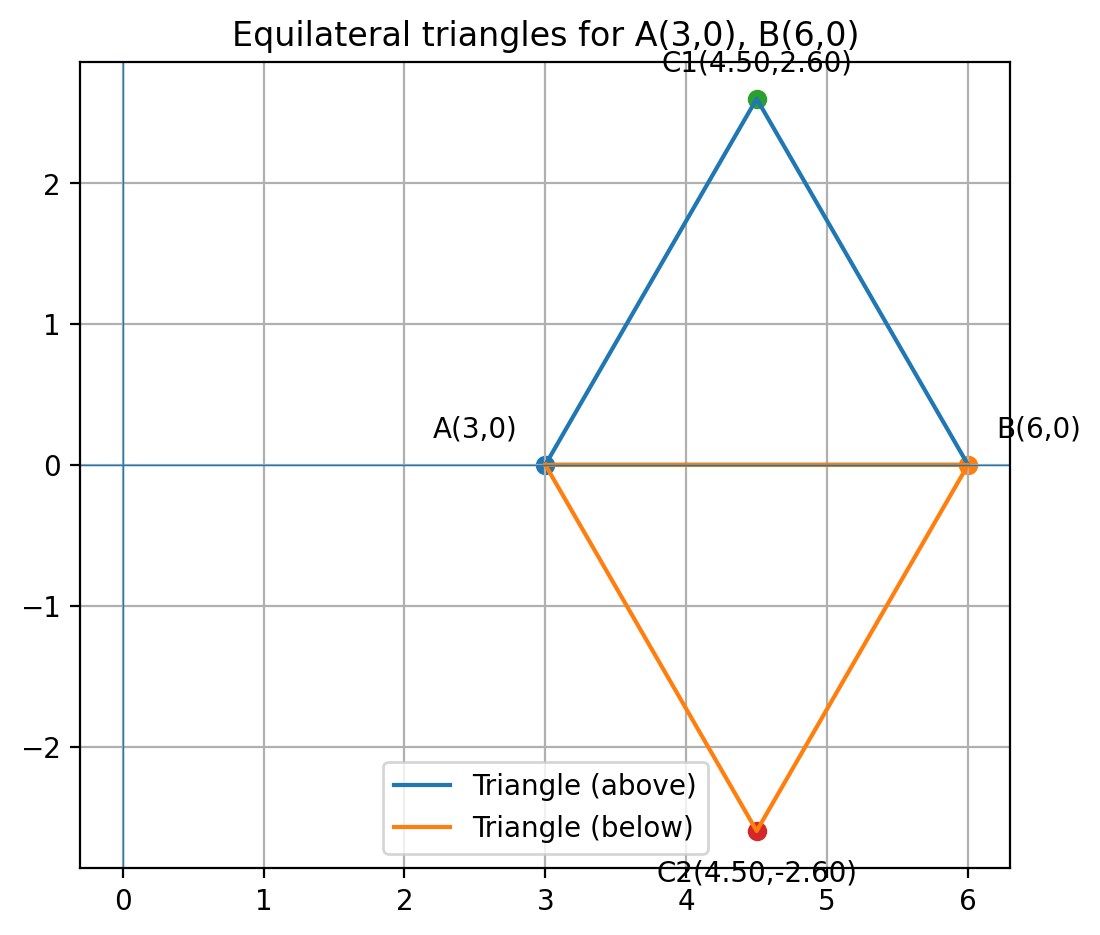
\includegraphics[width=0.4\columnwidth]{figs/01.png}
    \label{fig-1}
\end{figure}
   


   

\end{document}
